
\chapter{P-TOPO程序结构与ADS注入器I模拟}
\label{chap:PTOPO_ADS}

粒子云网格(Paticle-In-Cell, PIC)方法是研究空间电荷效应非常常用的的一种数值模拟算法\cite{PIC_birdsall2004plasma,PIC_luccio2002space}。PIC发展于上世纪七十年代,被广泛的应用于等离子体模拟和加速器设计。随着加速器的流强越来越高,束流模拟代码在束流动力学研究中的作用也越来越重要,尤其是在例如C-ADS,SNS,ESS等加速器中\cite{li2013physics,henderson2014spallation,eshraqi2016ess},其非线性空间电荷效应占据主导地位。一个拥有更强大的计算能力以及更高的精确度的程序,是我们研究强流束流动力学所必须的。我们开发了一个新的粒子模拟程序,命名为Parallel-Trace of Particle Orbits (P-TOPO),致力于研究强流加速器中的空间电荷效应问题\cite{li2016nonlinear,li2014envelope,li16collective,li2015space}。

在本章,我们首先介绍P-TOPO代码情况,之后使用P-TOPO对C-ADS进行模拟研究。

\section{程序结构}
P-TOPO使用C++语言开发,并且使用OpenMP进行并行化,目标是在普通多核PC机上快速模拟粒子在加速器中的行为。
P-TOPO使用时间t,而不是使用位置z,作为基本的独立变量,这是研究粒子的空间电荷效应非常自然的选择。即时使用位置z作为基本变量,在求解空间电荷力的过程中,也需要将粒子坐标转换为同一时间t下的时空间坐标。
在P-TOPO中,产生外场的一些加速器元件,例如各种磁铁,螺线管,RFQ,的外场使用元件的解析模型得到;而对于另外一些元件,例如超导腔,我们首先读取场文件\cite{studio2008cst},然后采用二阶插值的方法获取粒子所受到的场的大小和方向。
对于束团内部的空间电荷效应,我们使用经典的PIC方法进行求解\cite{hockney1988computer}。
程序的结构如图\ref{fig:P_TOPO}所示,图中每一个条目为一个类:
\begin{itemize}
  \item 主类MAIN调用其他各个具体的类,比如从外部Lattice结构中获取外场,求解内部空间电荷力,以及根据粒子所受的场推动粒子的位置和动量。
  \item Lattice类根据外部输入文件,解析或者数值地构建加速器的结构,以及根据粒子坐标,给出粒子所受的外场力。
  \item Distribution类产生粒子的初始分布,目前可以产生 KV,Waterbag,Parabolic,和Gaussian四种粒子分布,如图\ref{fig:distribution}所示。
  \item Beam类统计粒子的信息,并且计算出如rms大小,发射度等束团参数,将其保存以供进一步分析和输出。
  \item Internal Field类通过PIC方法计算空间电荷效应,在PIC方法中,我们使用FFT来求解Poisson方程。
  \item Leapfrog类和Runge-Kutta 4类都是继承Pusher类,是不同的推动粒子位置和动量的方法。
\end{itemize}

\begin{figure}[!htb]
    \centering
    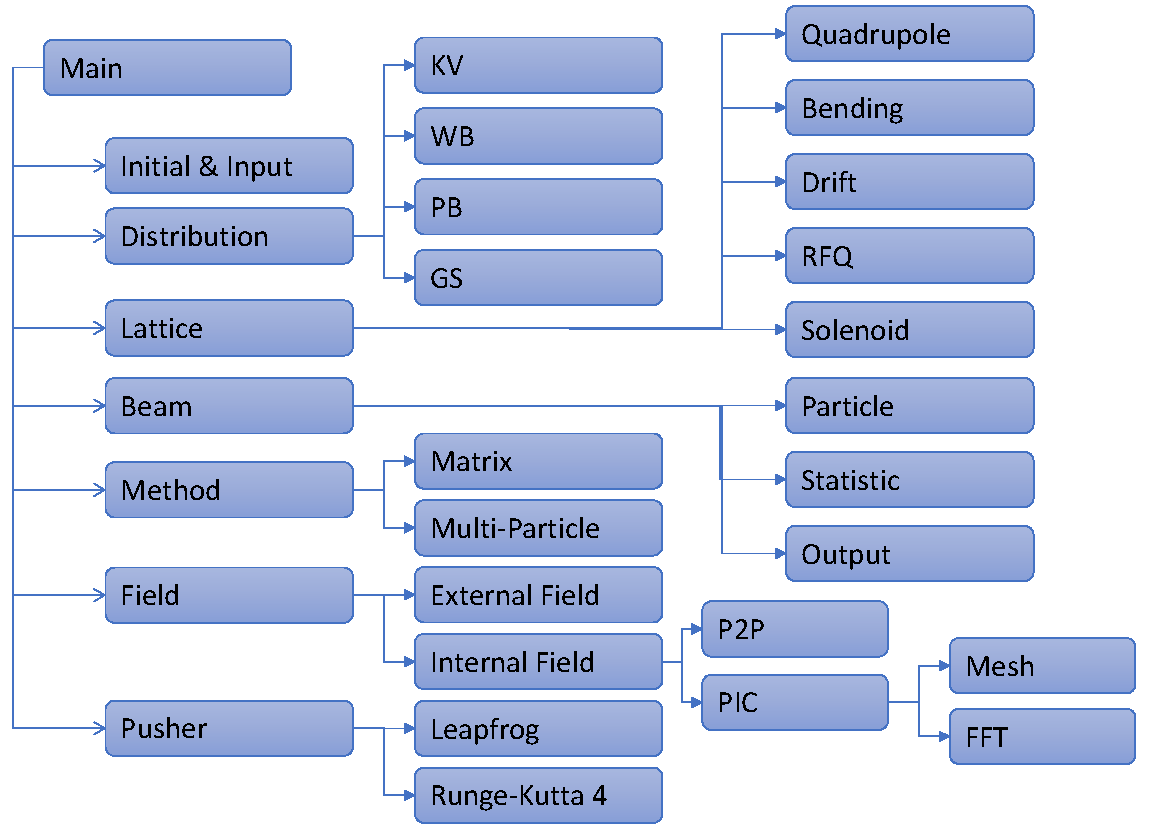
\includegraphics[width=0.8\textwidth]{Img/P_TOPO.pdf}
    \caption{P-TOPO程序结构}
    \label{fig:P_TOPO}
\end{figure}

\begin{figure}[!htb]
    \centering
    \begin{subfigure}[b]{0.48\textwidth}
        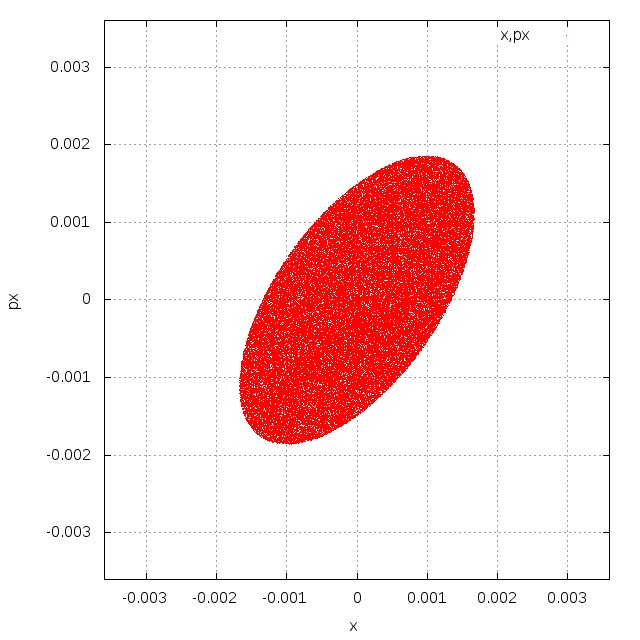
\includegraphics[width=\textwidth]{Img/KV_x_dx.jpg}
        \caption{KV}
    \end{subfigure}
    \begin{subfigure}[b]{0.48\textwidth}
        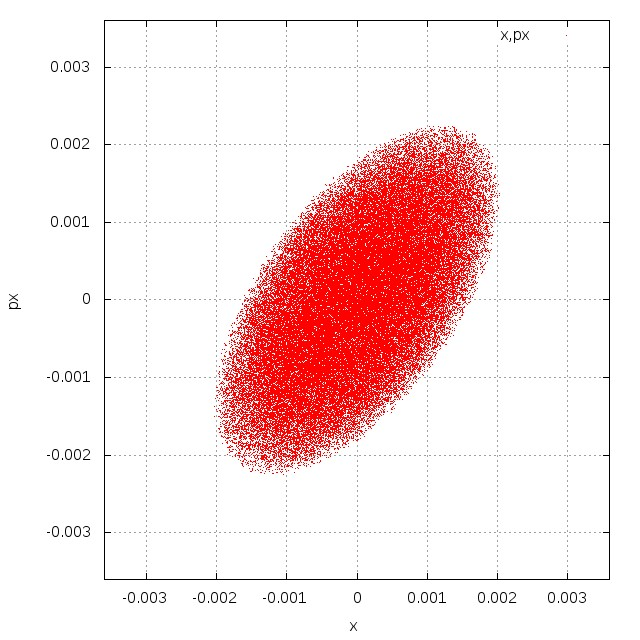
\includegraphics[width=\textwidth]{Img/WB_x_dx.jpg}
        \caption{Waterbag}
    \end{subfigure}
    \begin{subfigure}[b]{0.48\textwidth}
        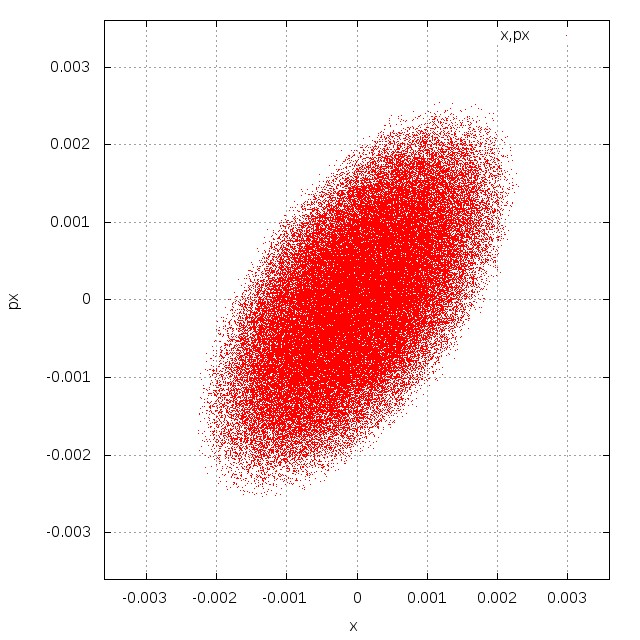
\includegraphics[width=\textwidth]{Img/PB_x_dx.jpg}
        \caption{Parabolic}
    \end{subfigure}
    \begin{subfigure}[b]{0.48\textwidth}
        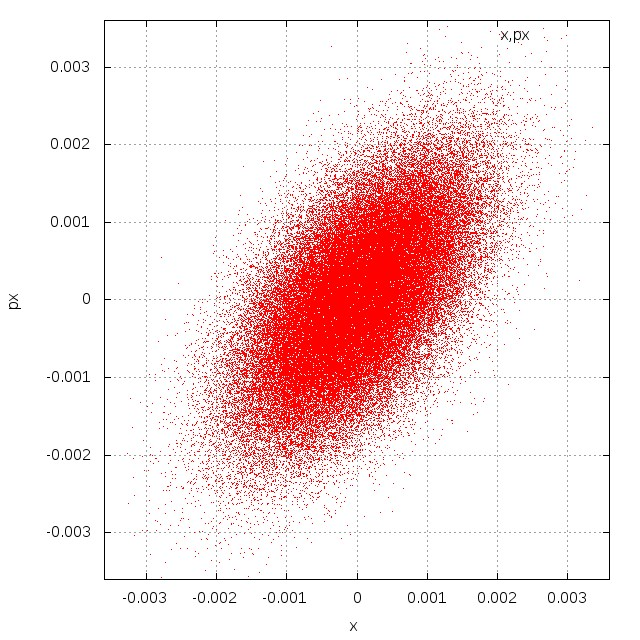
\includegraphics[width=\textwidth]{Img/GS_x_dx.jpg}
        \caption{Gaussian}
    \end{subfigure}
    \caption{同一均方根尺寸下的不同种类束团分布}\label{fig:distribution}
\end{figure}

程序主循环中的大部分都是并行化的,例如求解内场,推动粒子等。
最基本的,程序采用粒子并行策略,即每个线程处理不同的粒子。以粒子推动部分为例,如果粒子总数为160000,线程数为8,那么每个线程推动20000个粒子。
程序对可能发生线程冲突的部分,例如权重粒子,采用了其他的并行策略。除此之外,程序也使用了FFTW库的内部并行方法。


%程序也采用了一些其他的并行策略,以PIC求解Poisson方程为例,这部分需要4个独立的步骤来得到内部空间电荷场:
%\begin{enumerate}
%  \item 将粒子权重到网格,获得网格上的电荷密度;
%  \item 通过FFT求解网格上的Poisson方程,获得网格上的电势;
%  \item 对电势进行差分,获得网格上的电场;
%  \item 通过逆权重,得到粒子所在位置的电场。
%\end{enumerate}
%在第一步和第四步中,我们使用网格并行,即不同的线程处理不同的网格,这需要我们对粒子进行排序,以避免潜在的线程冲突。而在第二步和第三部中,主要的计算为傅里叶变换,程序使用了FFTW库的内部并行方法。

我们使用了一个4核的普通PC机进行性能测试,4线程运行的程序的速度是串行运行程序的3.6倍。关于程序的更大规模的并行问题,我们会在下一章做进一步讨论。
\section{正确性校验}
\subsection{内场计算}
我们使用一个点电荷来测试PIC部分的正确性。使用的格点数目为128*128*64。横向边界为狄利克雷边界条件(第一类边界条件),纵向为周期性边界条件。
图\ref{fig:P_TOPO_verification1}是P-TOPO的结果与理论值的对比,其中左图为横向电势(X方向),右图为纵向电势(Z方向)。图中红色实线为程序通过PIC方法计算得到的电势场的大小,绿色虚线为理论值,可以看出,程序的结果与理论值非常吻合。

\begin{figure}[!htb]
    \centering
    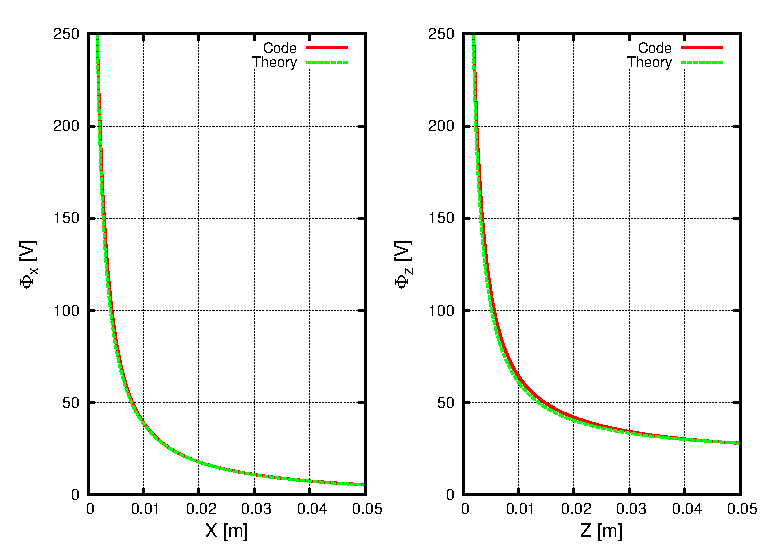
\includegraphics[width=0.8\textwidth]{Img/P_TOPO_verification1.eps}
    \caption{P-TOPO与理论值的点电荷电势对比}
    \label{fig:P_TOPO_verification1}
\end{figure}

\subsection{FD结构中与解析解的对比}
我们以束流在FD结构中束流的演化为例,来验证P-TOPO程序整体的正确性。连续束在周期聚焦结构中的束流包络方程可以表示为式\ref{eq:envelope}\cite{wangler1998particle,chen1994nonlinear}
\begin{equation}\label{eq:envelope}
  \frac{{{d}^{2}}R}{d{{z}^{2}}}+k_{0}^{2}R-\frac{{{\varepsilon }^{2}}}{{{R}^{3}}}-\frac{K}{R}=0
\end{equation}
其中$R$是束流横向均方根尺寸,$k_0$是聚焦强度,与外场力相关,$\varepsilon$为发射度,$K$是空间电荷力强度。束流的横向均方根尺寸与初始匹配和相移有关。
在这个验证中,计算空间电荷力的网格数目为64*64,我们使用10000个宏粒子在KV初始分布下,分别以0mA和15mA在周期性FD结构中前进,每个FD结构中推动400步。
图\ref{fig:P_TOPO_verification2}显示了由P-TOPO给出的束流均方根尺寸的演变和均方根包络方程的理论预期,其中图片下部浅蓝色线表示外部四级铁的聚焦强度,红色实线和绿色虚线分别为零流强下理论结果和P-TOPO程序计算结果,而蓝色实线和紫色虚线分别代表15mA流强下理论预期和P-TOPO计算结果。可以看出,无论是在零流强时还是15mA流强时,计算结果与理论值都保持高度一致,其中在15mA下束团演变的微小区别是因为包络方程计算中假定发射度为常数,而实际的PIC计算中发射度会发生变化。

\begin{figure}[!htb]
    \centering
    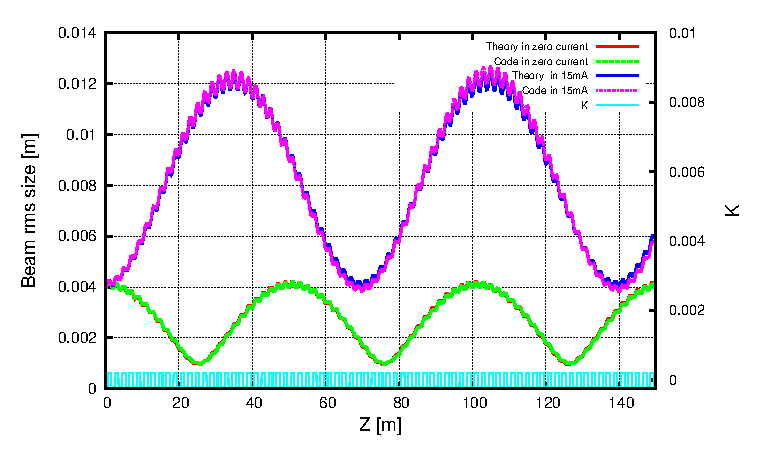
\includegraphics[width=0.8\textwidth]{Img/P_TOPO_verification2.eps}
    \caption{零流强和15mA时,P-TOPO结果与包络方程的对比}
    \label{fig:P_TOPO_verification2}
\end{figure}

\section{C-ADS注入器I模拟}

我们使用P-TOPO代码模拟了C-ADS的注入器I。加速器驱动次临界洁净核能系统(Accelerator Driven Sub-critical System,ADS),是一种新型的能源装置,其基本原理是利用经过加速器加速的高能质子,撞击重靶核发生反应,一个质子引起的散裂反应可产生几十个中子,再使用散裂产生的中子作为中子源来驱动次临界包层系统,使次临界包层系统维持链式反应以便得到能量和利用多余的中子增殖核材料和嬗变核废物,其中中国ADS(C-ADS)的加速器部分由中国科学院高能物理研究所和近代物理研究所共同研究。C-ADS的注入器I由离子源(electron cyclotron resonance ion-source,ECRIS),低能传输线,RFQ,中能传输线,两个超导加速模块,以及最后的垃圾桶组成,其结构如图\ref{fig:ADS_layout}所示

\begin{figure}[!htb]
    \centering
    
\includegraphics[width=1.05\textwidth]{Img/Layout_of_ADS_Injector_I.jpg}
    \caption{C-ADS注入器I结构示意图}
    \label{fig:ADS_layout}
\end{figure}

C-ADS注入器I的基本参数如表\ref{tab:C_ADS_parameters}所示。其中RFQ是使用PARMTEQM\cite{crandall1998rfq}设计的,频率为325MHz,将10mA的质子束流从35keV加速到3.2MeV,并且以后有可能升级到15mA。因为注入能量较低,只有35keV,RFQ的参数和聚束节使用绝热设计以降低空间电荷效应的影响,这导致了最终较小的纵向发射度。RFQ之后是超导加速腔,经过14个Spoke腔将束流加速到最终的10MeV。

\begin{table}[!htbp]
    \centering
    \footnotesize% fontsize
    \setlength{\tabcolsep}{4pt}% column separation
    \renewcommand{\arraystretch}{1.2}%row space
    \begin{tabular}{lc}
        \hline\hline
        Particle                & Proton \\
        \hline
        Rf frequency (MHz)      & 325       \\
        \hline
        Injection energy (MeV)  & 0.035     \\
        \hline
        Output energy (MeV)     & 10        \\
        \hline
        Pulsed beam current (mA)& 10        \\
        \hline
        Beam duty factor        & 100\%     \\
        \hline
        Input normalized rms emittance X ($\pi$ mm mrad)    & 0.2        \\
        \hline
        Input normalized rms emittance Y ($\pi$ mm mrad)    & 0.2        \\
        \hline\hline
    \end{tabular}
    \caption{C-ADS注入器I基本参数}
    \label{tab:C_ADS_parameters}
\end{table}

我们对RFQ和后面的超导段分别进行模拟,宏粒子数目为20000个,横向初始分布使用KV分布,纵向初始分布为均匀分布。使用实际运行的加速器结构,并且当粒子的横向位置触碰元件的孔径后标记为丢失,其中RFQ稍微严格对待,其孔径为当前cell的最小半径。空间电荷效应的网格数为64*64*64(x/y/z)。在RFQ段,我们不但使用P-TOPO程序,同时也使用Track程序\cite{aseev2005track},以相同的初始条件进行模拟;同样的,在超导段,除了P-TOPO之外,我们还使用TraceWin\cite{uriot2014tracewin}来进行研究和对比。下面,我们对RFQ和超导段分别进行讨论。

\subsection{RFQ模拟}
在RFQ模拟中,RFQ中的场可由傅里叶贝塞尔方程的八项式得到,如式\ref{eq:RFQ_8terms}:
\begin{equation}
    \begin{aligned}
       {{U}_{ex}}(r,\theta ,z) & =\frac{V}{2}[{{A}_{01}}{{(r/{{r}_{0}})}^{2}}\cos (2\theta )+{{A}_{10}}{{I}_{0}}(kr)\cos (kz) \\
     & +{{A}_{03}}{{(r/{{r}_{0}})}^{6}}\cos (6\theta )+{{A}_{21}}{{I}_{2}}(2kr)\cos (2\theta )\cos (2kz) \\
     & +{{A}_{12}}{{I}_{4}}(kr)\cos (4\theta )\cos (kz)+{{A}_{03}}{{I}_{0}}(3kr)\cos (3kz) \\
     & +{{A}_{23}}{{I}_{6}}(2kr)\cos (6\theta )\cos (2kz)+{{A}_{32}}{{I}_{4}}(3kr)\cos (4\theta )\cos (3kz)]
    \end{aligned}
    \label{eq:RFQ_8terms}
\end{equation}
其中$I_n$为第n阶修正贝塞尔方程,$k=\pi /2\beta \gamma$,$A_mn$系数由RFQ设计程序PARMTEQM给出。

图\ref{fig:ADS_RFQ_emit}是P-TOPO和TRACK在0mA下和15mA下对RFQ模拟得到的横向和纵向发射度演化,其中红色实线为P-TOPO的结果而绿色虚线为TRACK的结果。在横向和纵向两个方向上,P-TOPO的发射度演变结果都更加光滑,尤其是在RFQ的前端。在此处,束流开始丝化形成束团,并且相空间开始剧烈旋转。P-TOPO与TRACK的结果误差在合理范围内。

\begin{figure}[!htb]
    \centering
    \begin{subfigure}[b]{0.9\textwidth}
        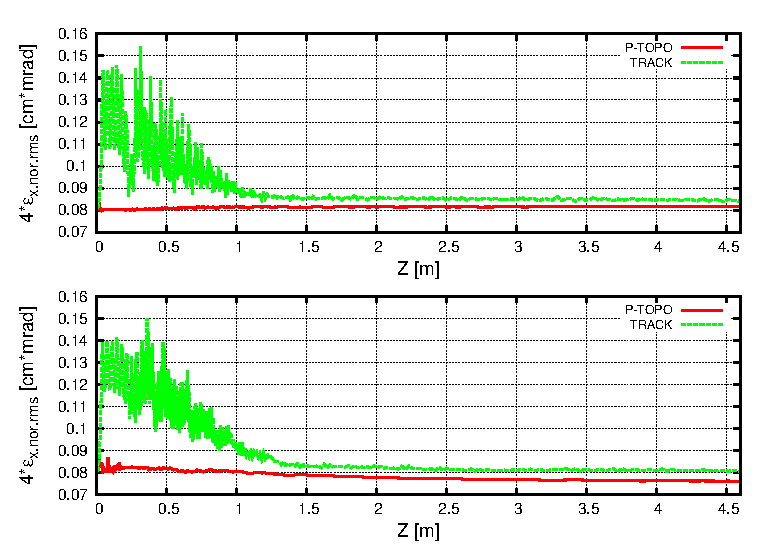
\includegraphics[width=\textwidth]{Img/ADS_RFQ_emit1.eps}
        \caption{0mA(上)和15mA(下)时RFQ中的横向发射度}
    \end{subfigure}
    \begin{subfigure}[b]{0.9\textwidth}
        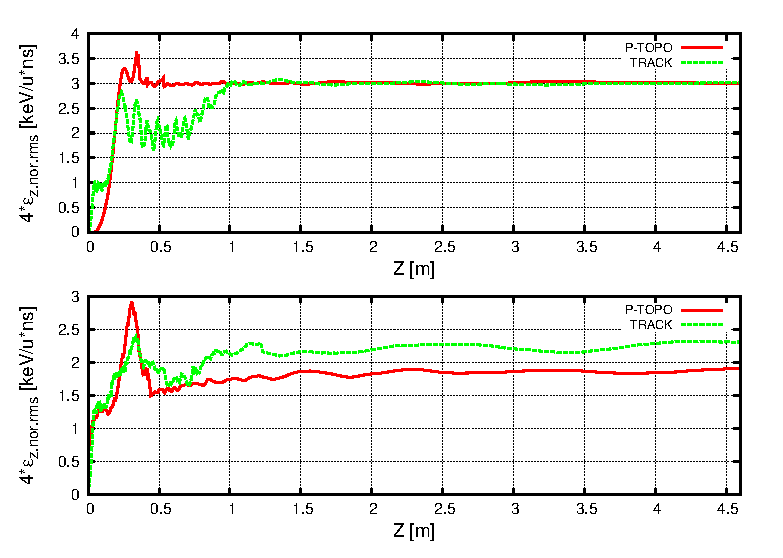
\includegraphics[width=\textwidth]{Img/ADS_RFQ_emit2.eps}
        \caption{0mA(上)和15mA(下)时RFQ中的纵向发射度}
    \end{subfigure}
    \caption{RFQ中的横向发射度和纵向发射度}\label{fig:ADS_RFQ_emit}
\end{figure}



图\ref{fig:ADS_RFQ_size1}是P-TOPO和TRACK在15mA下对RFQ模拟得到的横向束团尺寸演化,图\ref{fig:ADS_RFQ_size2}是P-TOPO和TRACK在15mA下对RFQ模拟得到的纵向束团尺寸和能散演化,其中红色实线为P-TOPO的结果而绿色虚线为TRACK的结果。两个程序在束团均方根尺寸上吻合得很好,其差别在合理范围内。同时验证了C-ADS注入器I的RFQ设计能够有效的控制束团的发射度和尺寸。

\begin{figure}[!htb]
    \centering
    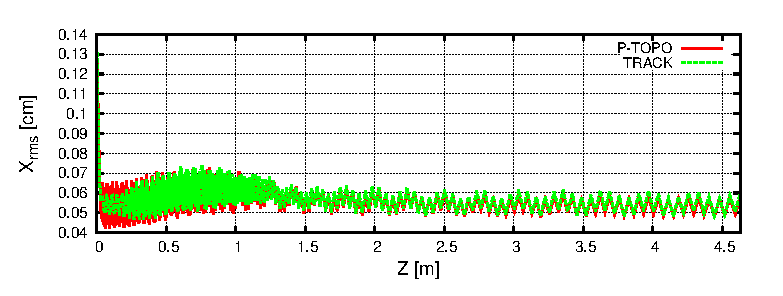
\includegraphics[width=0.9\textwidth]{Img/ADS_RFQ_size1.eps}
    \caption{RFQ中束团横向均方根尺寸}
    \label{fig:ADS_RFQ_size1}
\end{figure}

\begin{figure}[!htb]
    \centering
    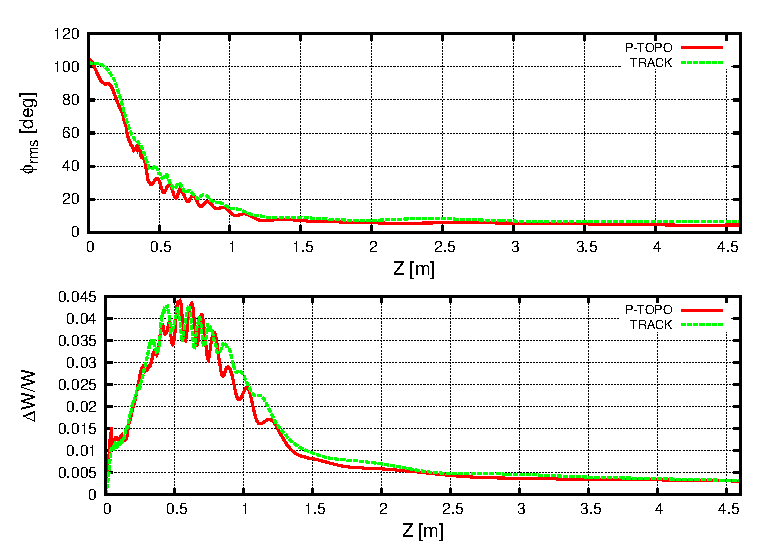
\includegraphics[width=0.9\textwidth]{Img/ADS_RFQ_size2.eps}
    \caption{RFQ中束团纵向均方根尺寸和能散}
    \label{fig:ADS_RFQ_size2}
\end{figure}

\subsection{超导段模拟}
在超导段中,聚束腔和加速腔的场由文件导入,P-TOPO使用数值差值来得到粒子所受到的场强。在设计的15mA流强下,RFQ出口处3.2MeV的质子束流经过聚束,通过MEBT进入超导段,逐渐加速到10MeV。在超导段中我们使用P-TOPO和TraceWin来进行模拟。

图\ref{fig:ADS_SC_emit}为P-TOPO和TraceWin在15mA下对RFQ模拟得到的横向和纵向发射度演化,其中红色实线为P-TOPO的结果而绿色虚线为TraceWin的结果。
两个程序得到的结果相一致。其中横向发射度除了在螺线管处有一个峰值外,基本保持不变。螺线管处的峰值是因为P-TOPO和TraceWin都是以时间t为基本变量,即发射度是由同一时刻的粒子信息统计得到,而不是由同一纵向位置的粒子得到,因此,在束团进入螺线管的时候,部分粒子先进入,部分粒子还没有进入,导致相空间的扭曲,从而导致统计发射度的突变。纵向发射度有略微增长,增长幅度在20\%以内。横纵向的发射度增长是由空间电荷力,磁铁边缘场的非线性效应,以及超导腔内的非线性纵向力导致,这几个驱动发射度增长的来源共同作用,使粒子相空间扭曲,最终会导致束晕的产生。P-TOPO的模拟中,出口能量为10.01MeV,而TraceWin的模拟出口能量为10.06MeV。
\begin{figure}[!htb]
    \centering
    \begin{subfigure}[b]{0.9\textwidth}
        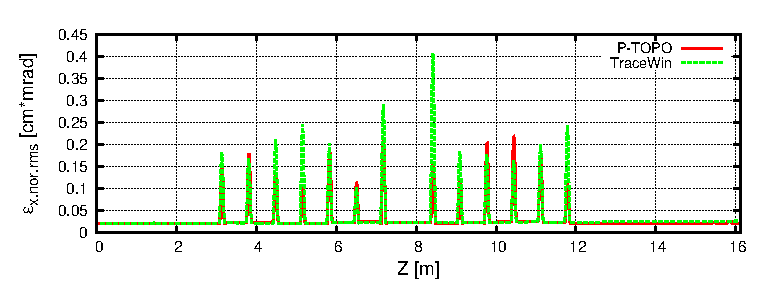
\includegraphics[width=\textwidth]{Img/ADS_SC_emit1.eps}
        %\caption{}
    \end{subfigure}
    \begin{subfigure}[b]{0.9\textwidth}
        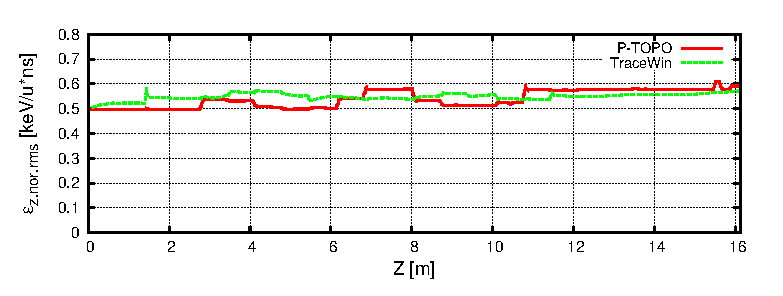
\includegraphics[width=\textwidth]{Img/ADS_SC_emit2.eps}
        %\caption{}
    \end{subfigure}
    \caption{超导段横向发射度和纵向发射度}\label{fig:ADS_SC_emit}
\end{figure}

图\ref{fig:ADS_SC_size}是P-TOPO和TraceWin在15mA下对超导段模拟得到的横纵向束团尺寸演化和能散演化,其中红色实线为P-TOPO的结果而绿色虚线为TRACK的结果。两个程序模拟结果的细微差别主要是因为两个程序获取同步相位的方法不同。TraceWin使用时间漂移法获得同步相位,而P-TOPO使用扫相获得同步相位。束团的横向尺寸相比管道半径都很小,而纵向尺寸也被聚束腔和接下来的各个加速腔有效地压缩,一般不会有束损出现。
\begin{figure}[!htb]
    \centering
    \begin{subfigure}[b]{0.9\textwidth}
        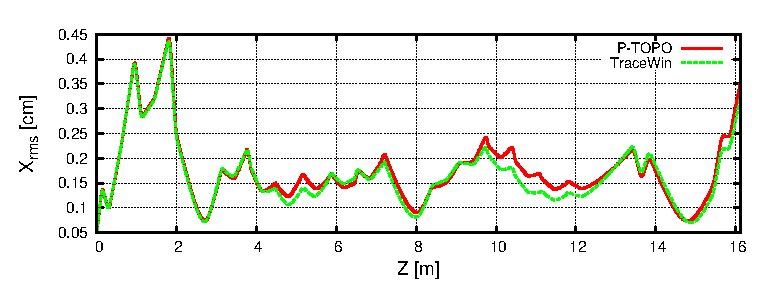
\includegraphics[width=\textwidth]{Img/ADS_SC_size1.eps}
        %\caption{}
    \end{subfigure}
    \begin{subfigure}[b]{0.9\textwidth}
        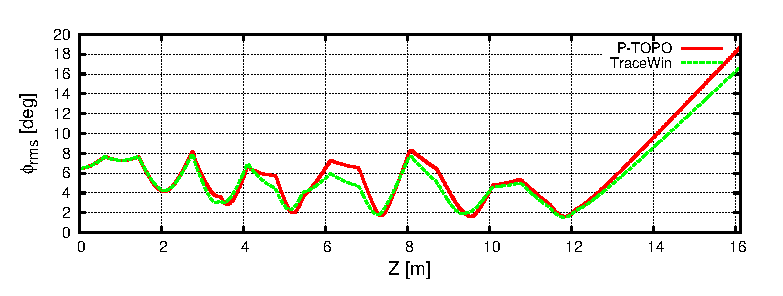
\includegraphics[width=\textwidth]{Img/ADS_SC_size2.eps}
        %\caption{}
    \end{subfigure}
    \begin{subfigure}[b]{0.9\textwidth}
        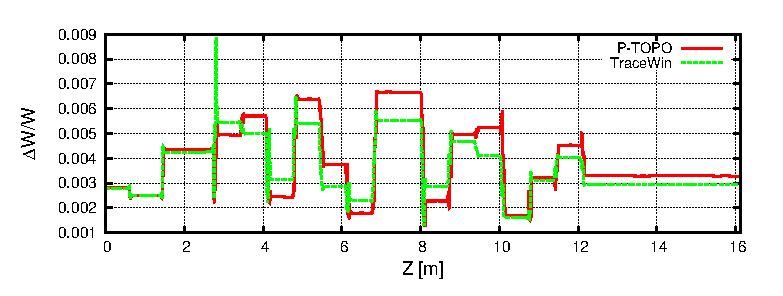
\includegraphics[width=\textwidth]{Img/ADS_SC_size3.eps}
        %\caption{}
    \end{subfigure}
    \caption{超导段束团横纵向尺寸以及能散}\label{fig:ADS_SC_size}
\end{figure}

在RFQ和超导段两段模拟中,传输效率都在99.9\%以上,束团尺寸和束损都得到了有效控制,横向和纵向的发射度都保持良好。不同代码的模拟结果差别主要是因为初始的束团分布不同,以及统计数据的方式不同,特别是P-TOPO是以时间t为基本变量,而TRACK是以位置z为基本变量,因此粒子信息收集,空间电荷力的计算,以及粒子推动方式都有所不同。

\section{小结}
我们在介绍了根据PIC算法编写的粒子模拟程序P-TOPO,主要处理强流加速器中的非线性效应。
P-TOPO的PIC部分和整体正确性都得到了验证,并应用在C-ADS注入器I的RFQ和超导段,分别对其进行了模拟并且与其他程序进行了比较。
模拟结果证明了现有设计的合理性,束团的尺寸和发射度都得到了有效控制,束损以及能散也在合理范围之内,完全满足需求。
之后,我们将继续对P-TOPO进行拓展并加入更多新的功能,以满足强流加速器的各种需求。